\documentclass{ximera}
\input{../preamble}

\addPrintStyle{..}

\begin{document}
	\author{Bart Lambregs}
	\xmtitle{Bewerkingen met vectoren}{}
    \xmsource\xmuitleg


% SCALAIRE VERMENIGVULDIGING 

% ph: maar met 1 shift vector doen; is veel simpelen -1*(Shift) is de andere
%  TIKZPICTURE DIE DE SCALAIRE VERMENIGVULDIGING ILLUSTREERT 
\begin{tikzpicture}
    % \draw (-4,-4) grid (4,4);

    \pgfmathsetmacro{\ax}{2}  
    \pgfmathsetmacro{\ay}{0}  

    % \pgfmathsetmacro{\c}{$\sqrt{2}$}  
    \pgfmathsetmacro{\d}{2} 

    \coordinate (O) at (0,0); 
    \coordinate (A) at (\ax,\ay); 
    
    \coordinate (Shift) at (0,0.1); 

    \fill (O) circle (2pt); %node[below left]{O};

    \draw[->, very thick,  -latex] (O) -- ($(A)$) node[midway, below]{\(\vec{a}\)};
    \draw[->, very thick,  -latex, blue] ($ (O) - (Shift)$) -- ($-1*(A) - (Shift)$) node[midway, above]{\(-\vec{a}\)};

    \draw[->, very thick,  -latex] ($ (O) + (Shift)$) -- ($\d*(A) + (Shift)$) node[midway, above]{\(2 \cdot \vec{a}\)};
    \draw[->, very thick,  -latex, blue] ($ (O) - 2*(Shift)$) -- ($-0.5*(A) - 2*(Shift)$) node[midway, below, red]{\(-\frac{1}{2}\vec{a}\)};

\end{tikzpicture}



% SOM EN VERSCHIL 

% TIKZPICTURE DIE DE SOM VAN TWEE VECTOREN BEREKENT 
\begin{tikzpicture}
    % \draw (-4,-4) grid (4,4);

    \pgfmathsetmacro{\ax}{1}  
    \pgfmathsetmacro{\ay}{2}  
    \pgfmathsetmacro{\bx}{3}  
    \pgfmathsetmacro{\by}{1} 

    \coordinate (O) at (0,0); 
    \coordinate (A) at (\ax,\ay); 
    \coordinate (B) at (\bx,\by); 

    \fill (O) circle (2pt) node[below left]{O};
    % \fill (A) circle (2pt);
    % \fill (B) circle (2pt);

    \draw[->, -latex] (O) -- (A) node[midway, below]{\(\vec{a}\)};
    \draw[->, -latex] (O) -- (B) node[midway, below]{\(\vec{b}\)};
    
    \draw[->, -latex, red, thick] (O) -- ($ (A) + (B)$) node[midway, below]{\(\vec{a} + \vec{b}\)};
    \draw[->, dashed, -latex, red, thick] (A) -- ($ (A) + (B)$) node[midway, below]{\( \vec{b} \)};
    \draw[->, dashed, -latex, red, thick] (B) -- ($ (A) + (B)$) node[midway, below]{\( \vec{a} \)};

\end{tikzpicture}



% ONTBINDEN IN COMPONENTEN 


% TIKZPICTURE DIE DE ONTBINDING IN COMPONENTEN WEERGEEFT 
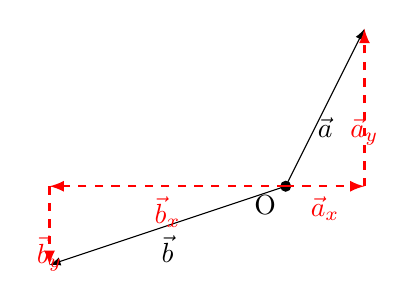
\begin{tikzpicture}
    % \draw (-4,-4) grid (4,4);

    \pgfmathsetmacro{\ax}{1}  
    \pgfmathsetmacro{\ay}{2}  
    \pgfmathsetmacro{\bx}{-3}  
    \pgfmathsetmacro{\by}{-1} 

    \coordinate (O) at (0,0); 
    \coordinate (A) at (\ax,\ay); 
    \coordinate (B) at (\bx,\by); 

    \fill (O) circle (2pt) node[below left]{O};
    % \fill (A) circle (2pt);
    % \fill (B) circle (2pt);


    \draw[->, -latex] (O) -- (A) node[midway, below]{\(\vec{a}\)};
    \draw[->, dashed, -latex, red, thick] (O) -- (\ax, 0) node[midway, below]{\( \vec{a}_x \)};
    \draw[->, dashed, -latex, red, thick] (\ax, 0) -- (A) node[midway, below]{\( \vec{a}_y \)};
    
    
    \draw[->, -latex] (O) -- (B) node[midway, below]{\(\vec{b}\)};
    \draw[->, dashed, -latex, red, thick] (O) -- (\bx, 0) node[midway, below]{\( \vec{b}_x \)};
    \draw[->, dashed, -latex, red, thick] (\bx, 0) -- (B) node[midway, below]{\( \vec{b}_y \)};
    
\end{tikzpicture}


% SCALAIR PRODUCT 

% TIKZPICTURE DIE SCALAIR PRODUCT van a op b ILLUSTREERT  
\begin{tikzpicture}
    % \draw (-4,-4) grid (4,4);

    \pgfmathsetmacro{\ax}{1}  
    \pgfmathsetmacro{\ay}{2}  
    \pgfmathsetmacro{\bx}{3}  
    \pgfmathsetmacro{\by}{0} 

    \coordinate (O) at (0,0); 
    \coordinate (A) at (\ax,\ay); 
    \coordinate (B) at (\bx,\by); 

    \fill (O) circle (2pt) node[below left]{O};
    
    \draw[->, -latex] (O) -- (B) node[midway, below]{\(\vec{b}\)};

    \draw[->, -latex] (O) -- (A) node[midway, above left]{\(\vec{a}\)};
    \draw[->, dashed, -latex, red, thick] (O) -- (\ax, 0) node[midway, below]{\( \vec{a}_x \)};
    \draw[dashed, -latex, thick] (\ax, 0) -- (A);


    \draw pic[ pic text= $\theta$, draw,  angle radius=0.7cm]{angle = B--O--A};
    
        
\end{tikzpicture}


% VECTORIEEL PRODUCT 

\end{document}
